\section{Machine Learning}
\paragraph{Références} \cite{AlphaGo0} \cite{AlphaGo1} \cite{Internet3} \cite{Internet4} \cite{Internet5}

\paragraph{Différences et similitudes avec IA} En quoi consiste le ML ? Bien qu'il soit
directement lié à l'IA, quelles sont ses différences et ses similitudes avec cette dernière ?

\paragraph{Une machine capable d'apprendre}

\paragraph {} Commençons par nous arrêter un instant sur le terme de \emph{Machine Learning}. En français,
cela pourrait se traduire par \emph{L'apprentissage de la machine}. Mais quel apprentissage ? N'est-ce pas
le rôle de l'Homme, comme nous l'avons soutenu jusqu'ici, d'apprendre à la machine ? Nous verrons que dans
le cas du Machine Learning, le concepteur ne fait que \emph{construire un système}, et lui donner
\emph{les clés} pour parvenir à la résolution d'un \emph{problème complexe}. On remarque ici l'importance
de \emph{cibler} un domaine: lorsque nous parlons de ML, nous ne prétendons pas créer un système à l'image
humaine, qui serait capable d'avoir une faculté d'apprentissage \emph{globale}, quelque soit le support. 

\paragraph{} Justement, n'est-ce pas là une réelle différence entre l'apprentissage humain et celui de la machine ?
Lorsque l'Homme apprend, c'est par \emph{l'expérience}. Il fait l'expérience de son environnement et la
conséquence de l'action lui permet d'être \emph{mieux préparé} à la prochaine expérience. Mais c'est en fait un
comportement similaire qui est utilisé en Machine Learning : un agent est entraîné à partir d'un certain nombre
d'entrées, dont il tire une sortie. Ce résultat est comparé à celui qui était attendu, puis la machine est
\emph{reparamétrée}, de sorte à ce qu'une prochaine expérience similaire aboutisse à un résultat plus proche 
de celui escompté. Ce processus de reconfiguration par l'apprentissage intervient notamment au niveau du cerveau
chez l'Homme, ce qui est concrétisé en, ML par l'utilisation de Réseaux Neuronaux ou Neural Networks (NN), dont
nous détaillerons l'utilisation par la suite. Ce qu'il faut retenir de la différence entre la méthode d'apprentissage
d'un Homme et d'une machine, c'est la capacité d'adaptation du tissu neuronal de l'Homme à une variété de situations
et de problèmes que la machine n'est pas capable d'appréhender seule.

\paragraph{Cerveau humain et Ordinateur}

\paragraph{} Afin de comprendre ces différences entre les capacités de l'Homme et de la machine, il nous faut nous
intéresser un instant à leur composition et à leur mode de fonctionnement. Rappelons en premier lieu qu'une machine
fonctionne sur un \emph{système binaire}, qu'elle est la seule à pouvoir comprendre. L'Homme de son côté réfléchit
par une infinité \emph{d'associations de sensations}, qui partent de son expérience sensorielle par les 5 sens : vue,
toucher, odorat, ouïe, goût. En ce sens la \emph{réflexion} est le propre de l'Homme, car il est seul à pouvoir 
apprendre par la projection de son expérience. \cite{Internet5}

\paragraph{} De plus, le cerveau humain possède une centaine de milliards de neurones, eux-mêmes connectés à plus de 10.000
de leurs voisins. Cette structure gigantesque n'est pas encore égalée par l'ordinateur, dont le nombre de cellules est de
l'ordre de 5 milliards, et dont les cellules sont contigües en mémoire. On remarquera néanmoins que l'information y circule
beaucoup plus rapidement que dans le cerveau, où les impulsions synaptiques atteignent 6 à 10 m/s. Enfin on remarquera que la
nature des mémoires est totalement différente : là où l'ordinateur est capable de \emph{stocker de l'information}, et est donc
capable de restituer une information de manière \emph{infaillible}, l'Homme doit compter sur les mémoires à court et long termes,
ainsi que sur ses registres sensoriels - ce qu'il connait de \emph{l'expérience}. \cite{Internet4}

\begin{figure}[h]
    \centering
    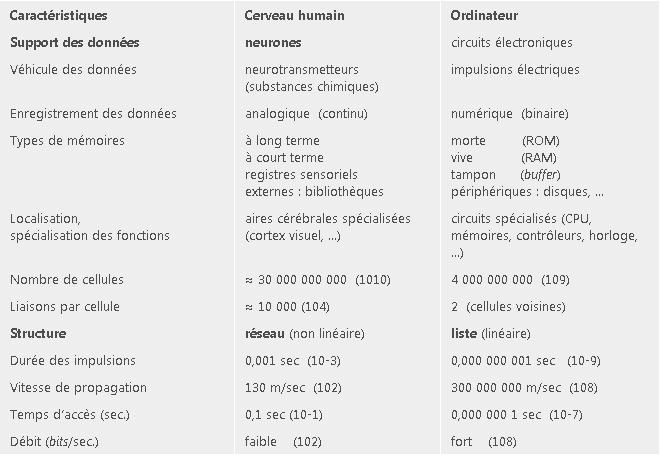
\includegraphics[width=350px]{chapters/03/images/cerveau-robot.jpg}
    \caption{\label{comparatif} \emph{Comparaison entre cerveau humain et ordinateur}, \url{http://intelligence-artificielle-tpe.e-monsite.com/pages/limites-technologiques-et-ethique-de-l-ia/cerveau-humain-et-robot.html}}
\end{figure}

\paragraph{Evolution logique et inévitable de l'IA} 

\paragraph{Systèmes intelligents} Lorem ipsum
